\documentclass[12pt]{beamer}\usepackage[]{graphicx}\usepackage[]{color}
%% maxwidth is the original width if it is less than linewidth
%% otherwise use linewidth (to make sure the graphics do not exceed the margin)
\makeatletter
\def\maxwidth{ %
  \ifdim\Gin@nat@width>\linewidth
    \linewidth
  \else
    \Gin@nat@width
  \fi
}
\makeatother

\definecolor{fgcolor}{rgb}{0.345, 0.345, 0.345}
\newcommand{\hlnum}[1]{\textcolor[rgb]{0.686,0.059,0.569}{#1}}%
\newcommand{\hlstr}[1]{\textcolor[rgb]{0.192,0.494,0.8}{#1}}%
\newcommand{\hlcom}[1]{\textcolor[rgb]{0.678,0.584,0.686}{\textit{#1}}}%
\newcommand{\hlopt}[1]{\textcolor[rgb]{0,0,0}{#1}}%
\newcommand{\hlstd}[1]{\textcolor[rgb]{0.345,0.345,0.345}{#1}}%
\newcommand{\hlkwa}[1]{\textcolor[rgb]{0.161,0.373,0.58}{\textbf{#1}}}%
\newcommand{\hlkwb}[1]{\textcolor[rgb]{0.69,0.353,0.396}{#1}}%
\newcommand{\hlkwc}[1]{\textcolor[rgb]{0.333,0.667,0.333}{#1}}%
\newcommand{\hlkwd}[1]{\textcolor[rgb]{0.737,0.353,0.396}{\textbf{#1}}}%
\let\hlipl\hlkwb

\usepackage{framed}
\makeatletter
\newenvironment{kframe}{%
 \def\at@end@of@kframe{}%
 \ifinner\ifhmode%
  \def\at@end@of@kframe{\end{minipage}}%
  \begin{minipage}{\columnwidth}%
 \fi\fi%
 \def\FrameCommand##1{\hskip\@totalleftmargin \hskip-\fboxsep
 \colorbox{shadecolor}{##1}\hskip-\fboxsep
     % There is no \\@totalrightmargin, so:
     \hskip-\linewidth \hskip-\@totalleftmargin \hskip\columnwidth}%
 \MakeFramed {\advance\hsize-\width
   \@totalleftmargin\z@ \linewidth\hsize
   \@setminipage}}%
 {\par\unskip\endMakeFramed%
 \at@end@of@kframe}
\makeatother

\definecolor{shadecolor}{rgb}{.97, .97, .97}
\definecolor{messagecolor}{rgb}{0, 0, 0}
\definecolor{warningcolor}{rgb}{1, 0, 1}
\definecolor{errorcolor}{rgb}{1, 0, 0}
\newenvironment{knitrout}{}{} % an empty environment to be redefined in TeX

\usepackage{alltt}
\usepackage{tikz}

% make it pretty
% get rid of junk
\usetheme{default}
\usefonttheme[onlymath]{serif}
\beamertemplatenavigationsymbolsempty

% define a bunch of colors
\definecolor{offwhite}{RGB}{255,250,240}
\definecolor{gray}{RGB}{155,155,155}
\definecolor{foreground}{RGB}{80,80,80}
\definecolor{background}{RGB}{255,255,255}
%\definecolor{title}{RGB}{255,199,0}
\definecolor{title}{RGB}{89,132,212}
%\definecolor{subtitle}{RGB}{89,132,212}
\definecolor{subtitle}{RGB}{255,199,0}
\definecolor{hilit}{RGB}{248,117,79}
\definecolor{vhilit}{RGB}{255,111,207}
\definecolor{lolit}{RGB}{200,200,200}
\definecolor{lit}{RGB}{255,199,0}
\definecolor{mdlit}{RGB}{89,132,212}
\definecolor{link}{RGB}{248,117,79}

% a few color macros
\newcommand{\hilit}{\color{hilit}}
\newcommand{\vhilit}{\color{vhilit}}
\newcommand{\lit}{\color{lit}}
\newcommand{\mdlit}{\color{mdlit}}
\newcommand{\lolit}{\color{lolit}}

% use those colors
\setbeamercolor{titlelike}{fg=title}
\setbeamercolor{subtitle}{fg=subtitle}
\setbeamercolor{frametitle}{fg=gray}
%\setbeamercolor{structure}{fg=subtitle}
\setbeamercolor{structure}{fg=title}
\setbeamercolor{institute}{fg=lolit}
\setbeamercolor{normal text}{fg=foreground,bg=background}
\setbeamertemplate{itemize subitem}{{\textendash}}
\setbeamerfont{itemize/enumerate subbody}{size=\small}
\setbeamerfont{itemize/enumerate subitem}{size=\small}

% center title of slides
\setbeamertemplate{blocks}[rounded]
\setbeamertemplate{frametitle}[default][center]

% page number
\setbeamerfont{page number in foot}{size=\footnotesize}
\setbeamertemplate{footline}[frame number]

% default link color
\hypersetup{colorlinks, urlcolor={link}}

% a few macros
\newcommand{\code}[1]{\texttt{#1}}
\newcommand{\hicode}[1]{{\hilit \texttt{#1}}}
\newcommand{\locode}[1]{{\lolit \texttt{#1}}}
\newcommand{\bb}[1]{\begin{block}{#1}}
\newcommand{\eb}{\end{block}}
\newcommand{\bi}{\begin{itemize}}
\newcommand{\bbi}{\vspace{4pt} \begin{itemize} \itemsep8pt}
\newcommand{\ei}{\end{itemize}}
\newcommand{\bv}{\begin{verbatim}}
\newcommand{\ev}{\end{verbatim}}
\newcommand{\ig}{\includegraphics}
\newcommand{\subt}[1]{{\footnotesize \color{subtitle} {#1}}}
\newcommand{\ttsm}{\tt \small}
\newcommand{\ttfn}{\tt \footnotesize}
\newcommand{\figh}[2]{\centerline{\includegraphics[height=#2\textheight]{#1}}}
\newcommand{\figw}[2]{\centerline{\includegraphics[width=#2\textwidth]{#1}}}



%------------------------------------------------

\title{Introduction}
\subtitle{Intro to Data Visualization}
\author{\href{http://www.gastonsanchez.com}{Gaston Sanchez}}
\institute{\href{https://creativecommons.org/licenses/by-sa/4.0/}{\tt \scriptsize \color{foreground} CC BY-SA 4.0}}
\date{}
\IfFileExists{upquote.sty}{\usepackage{upquote}}{}
\begin{document}



% no page number in first slide
{
  \setbeamertemplate{footline}{} 
  \frame{\titlepage} 
}

%------------------------------------------------

\begin{frame}
\begin{center}
\Huge{\hilit{Motivation: \\
Anscombe Dataset}}
\end{center}
\end{frame}

%------------------------------------------------

\begin{frame}[fragile]
\frametitle{Motivation}

Consider some data (four pairs of variables)
\begin{knitrout}\footnotesize
\definecolor{shadecolor}{rgb}{0.969, 0.969, 0.969}\color{fgcolor}\begin{kframe}
\begin{verbatim}
    x1     y1  x2    y2  x3     y3  x4     y4
1   10   8.04  10  9.14  10   7.46   8   6.58
2    8   6.95   8  8.14   8   6.77   8   5.76
3   13   7.58  13  8.74  13  12.74   8   7.71
4    9   8.81   9  8.77   9   7.11   8   8.84
5   11   8.33  11  9.26  11   7.81   8   8.47
6   14   9.96  14  8.10  14   8.84   8   7.04
7    6   7.24   6  6.13   6   6.08   8   5.25
8    4   4.26   4  3.10   4   5.39  19  12.50
9   12  10.84  12  9.13  12   8.15   8   5.56
10   7   4.82   7  7.26   7   6.42   8   7.91
11   5   5.68   5  4.74   5   5.73   8   6.89
\end{verbatim}
\end{kframe}
\end{knitrout}

\end{frame}

%------------------------------------------------

\begin{frame}
\begin{center}
\large{\mdlit{What things would you like \\ to calculate for each variable?}}
\end{center}
\end{frame}

%------------------------------------------------

\begin{frame}[fragile]
\frametitle{Motivation}

\begin{knitrout}\scriptsize
\definecolor{shadecolor}{rgb}{0.969, 0.969, 0.969}\color{fgcolor}\begin{kframe}
\begin{verbatim}
##        x1             x2             x3             x4    
##  Min.   : 4.0   Min.   : 4.0   Min.   : 4.0   Min.   : 8  
##  1st Qu.: 6.5   1st Qu.: 6.5   1st Qu.: 6.5   1st Qu.: 8  
##  Median : 9.0   Median : 9.0   Median : 9.0   Median : 8  
##  Mean   : 9.0   Mean   : 9.0   Mean   : 9.0   Mean   : 9  
##  3rd Qu.:11.5   3rd Qu.:11.5   3rd Qu.:11.5   3rd Qu.: 8  
##  Max.   :14.0   Max.   :14.0   Max.   :14.0   Max.   :19
\end{verbatim}
\end{kframe}
\end{knitrout}

\begin{knitrout}\scriptsize
\definecolor{shadecolor}{rgb}{0.969, 0.969, 0.969}\color{fgcolor}\begin{kframe}
\begin{verbatim}
##        y1               y2              y3              y4        
##  Min.   : 4.260   Min.   :3.100   Min.   : 5.39   Min.   : 5.250  
##  1st Qu.: 6.315   1st Qu.:6.695   1st Qu.: 6.25   1st Qu.: 6.170  
##  Median : 7.580   Median :8.140   Median : 7.11   Median : 7.040  
##  Mean   : 7.501   Mean   :7.501   Mean   : 7.50   Mean   : 7.501  
##  3rd Qu.: 8.570   3rd Qu.:8.950   3rd Qu.: 7.98   3rd Qu.: 8.190  
##  Max.   :10.840   Max.   :9.260   Max.   :12.74   Max.   :12.500
\end{verbatim}
\end{kframe}
\end{knitrout}

\end{frame}

%------------------------------------------------

\begin{frame}
\begin{center}
\large{\mdlit{What things would you like to calculate \\ for each pair of variables (e.g. \code{x1, y1})?}}
\end{center}
\end{frame}

%------------------------------------------------

\begin{frame}[fragile]
\frametitle{Motivation}

\begin{knitrout}\footnotesize
\definecolor{shadecolor}{rgb}{0.969, 0.969, 0.969}\color{fgcolor}\begin{kframe}
\begin{alltt}
\hlkwd{cor}\hlstd{(anscombe}\hlopt{$}\hlstd{x1, anscombe}\hlopt{$}\hlstd{y1)}
\end{alltt}
\begin{verbatim}
## [1] 0.8164205
\end{verbatim}
\begin{alltt}
\hlkwd{cor}\hlstd{(anscombe}\hlopt{$}\hlstd{x2, anscombe}\hlopt{$}\hlstd{y2)}
\end{alltt}
\begin{verbatim}
## [1] 0.8162365
\end{verbatim}
\begin{alltt}
\hlkwd{cor}\hlstd{(anscombe}\hlopt{$}\hlstd{x3, anscombe}\hlopt{$}\hlstd{y3)}
\end{alltt}
\begin{verbatim}
## [1] 0.8162867
\end{verbatim}
\begin{alltt}
\hlkwd{cor}\hlstd{(anscombe}\hlopt{$}\hlstd{x4, anscombe}\hlopt{$}\hlstd{y4)}
\end{alltt}
\begin{verbatim}
## [1] 0.8165214
\end{verbatim}
\end{kframe}
\end{knitrout}

\end{frame}

%------------------------------------------------

\begin{frame}[fragile]
\frametitle{Motivation}

\bbi
  \item Mean of \code{x} values = 9
  \item Mean of \code{y} values = 7.5009091
  \item least squares equation: $y = 3 + 0.5x$
  \item Sum of squared errors: 110
  \item Correlation coefficient: 0.8164205
\ei

\end{frame}

%------------------------------------------------

\begin{frame}
\frametitle{Data Visualization}

Using only numerical reduction methods in data analysis is far too limiting

\end{frame}

%------------------------------------------------

\begin{frame}[fragile]
\frametitle{Why Graphics?}

Are you able to see any patterns, associations, relations?
\begin{knitrout}\scriptsize
\definecolor{shadecolor}{rgb}{0.969, 0.969, 0.969}\color{fgcolor}\begin{kframe}
\begin{verbatim}
##     x1     y1  x2    y2  x3     y3  x4     y4
## 1   10   8.04  10  9.14  10   7.46   8   6.58
## 2    8   6.95   8  8.14   8   6.77   8   5.76
## 3   13   7.58  13  8.74  13  12.74   8   7.71
## 4    9   8.81   9  8.77   9   7.11   8   8.84
## 5   11   8.33  11  9.26  11   7.81   8   8.47
## 6   14   9.96  14  8.10  14   8.84   8   7.04
## 7    6   7.24   6  6.13   6   6.08   8   5.25
## 8    4   4.26   4  3.10   4   5.39  19  12.50
## 9   12  10.84  12  9.13  12   8.15   8   5.56
## 10   7   4.82   7  7.26   7   6.42   8   7.91
## 11   5   5.68   5  4.74   5   5.73   8   6.89
\end{verbatim}
\end{kframe}
\end{knitrout}

{\small Famous dataset \code{"anscombe"} (four data sets)}
\end{frame}

%------------------------------------------------

\begin{frame}[fragile]
\frametitle{Why Graphics?}

How are these two variables associated?

\bigskip
What does these data values look like?
\begin{knitrout}\scriptsize
\definecolor{shadecolor}{rgb}{0.969, 0.969, 0.969}\color{fgcolor}\begin{kframe}
\begin{verbatim}
    x1     y1
1   10   8.04
2    8   6.95
3   13   7.58
4    9   8.81
5   11   8.33
6   14   9.96
7    6   7.24
8    4   4.26
9   12  10.84
10   7   4.82
11   5   5.68
\end{verbatim}
\end{kframe}
\end{knitrout}

\end{frame}

%------------------------------------------------

\begin{frame}[fragile]
\frametitle{}

\begin{knitrout}\footnotesize
\definecolor{shadecolor}{rgb}{0.969, 0.969, 0.969}\color{fgcolor}

{\centering 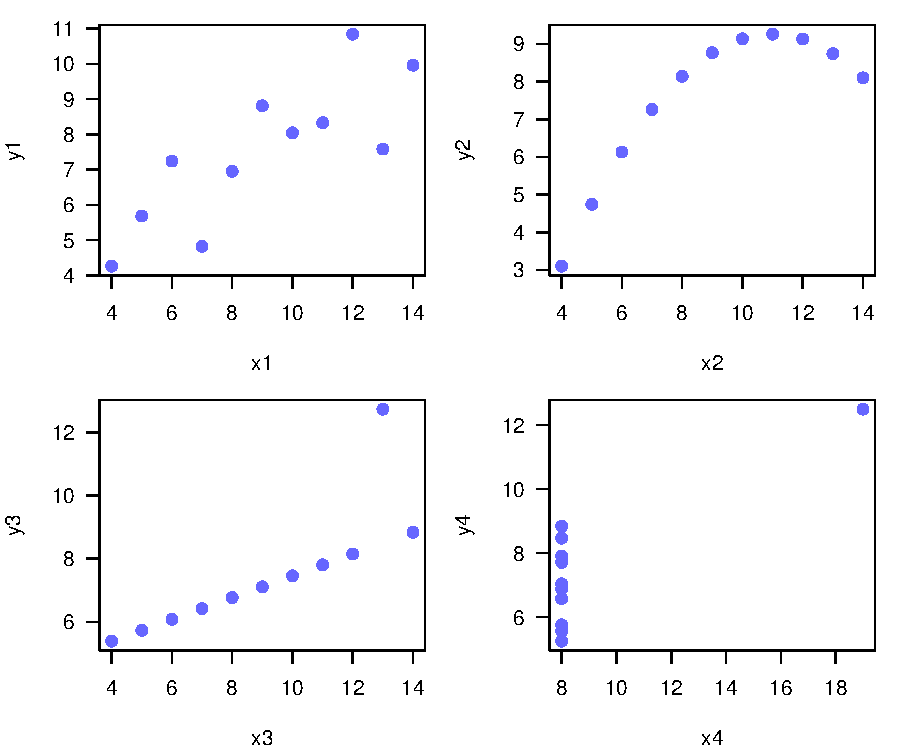
\includegraphics[width=.9\linewidth,height=.7\linewidth]{figure/unnamed-chunk-7-1} 

}



\end{knitrout}

\end{frame}

%------------------------------------------------

\begin{frame}
\begin{center}
\Huge{\hilit{Visualization}}
\end{center}
\end{frame}

%------------------------------------------------

{ % all template changes are local to this group.
    \begin{frame}[plain]
        \begin{tikzpicture}[remember picture,overlay]
            \node[at=(current page.center)] {
                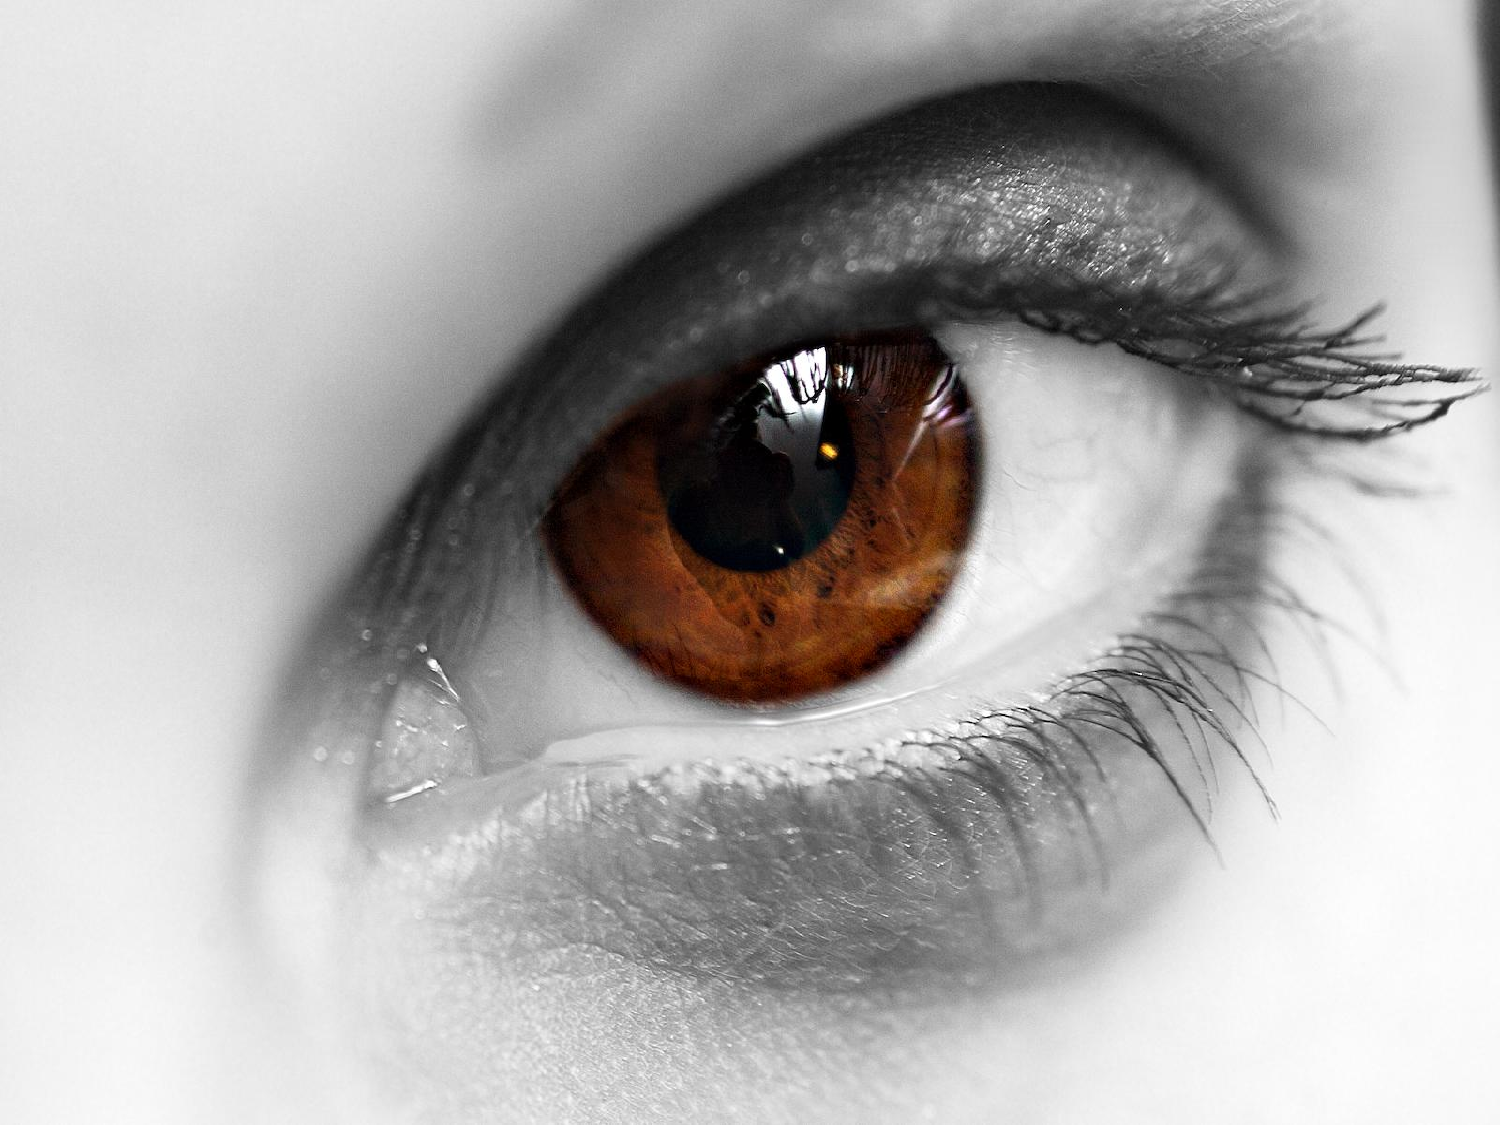
\includegraphics[width=\paperwidth]{images/eye-photo.pdf}
            };
        \end{tikzpicture}
     \end{frame}
}

%------------------------------------------------

\begin{frame}
\frametitle{Visualize}

\bb{Visualize}
\bbi
  \item To form a mental image of
  \item To make visible
\ei
\eb

\end{frame}

%------------------------------------------------

\begin{frame}
\frametitle{Visualization}

\Large Process of representing information or ideas by diagrams or graphs.

\textit{Ross Ihaka}

\end{frame}

%------------------------------------------------

\begin{frame}
\frametitle{Visualization}

\Large To convey information through visual representations

\end{frame}

%------------------------------------------------

\begin{frame}
\frametitle{What is visualization?}

\bb{Definition by OED}
The action or fact of visualizing; the power or process of forming
a mental picture or vision of something not actually present to the sight
\eb

\end{frame}

%------------------------------------------------

\begin{frame}
\frametitle{What is visualization?}

\bb{Definitions}
\bbi
  \item The action or process of rendering visible
  \item Transformation of the symbolic into the geometric 
  {\lolit McCormick et al 1987}
  \item The use of computer-generated, possibly interactive visual 
  representations of data to amplify cognition {\lolit Card, Mackinlay, \& Shneiderman 1999}
\ei
\eb

\end{frame}

%------------------------------------------------

\begin{frame}
\frametitle{What is visualization?}

\bb{Visualization}
Often referred to as the process of making a graphic or an image.
Actually it is a cognitive process
\eb

\end{frame}

%------------------------------------------------

\begin{frame}
\frametitle{Part of our language}

\bbi
  \item ``I see what you are saying''
  \item ``Seeing is believing''
  \item ``A picture is worth a thousand numbers''
\ei

\end{frame}

%------------------------------------------------

{ % all template changes are local to this group.
    \begin{frame}[plain]
        \begin{tikzpicture}[remember picture,overlay]
            \node[at=(current page.center)] {
                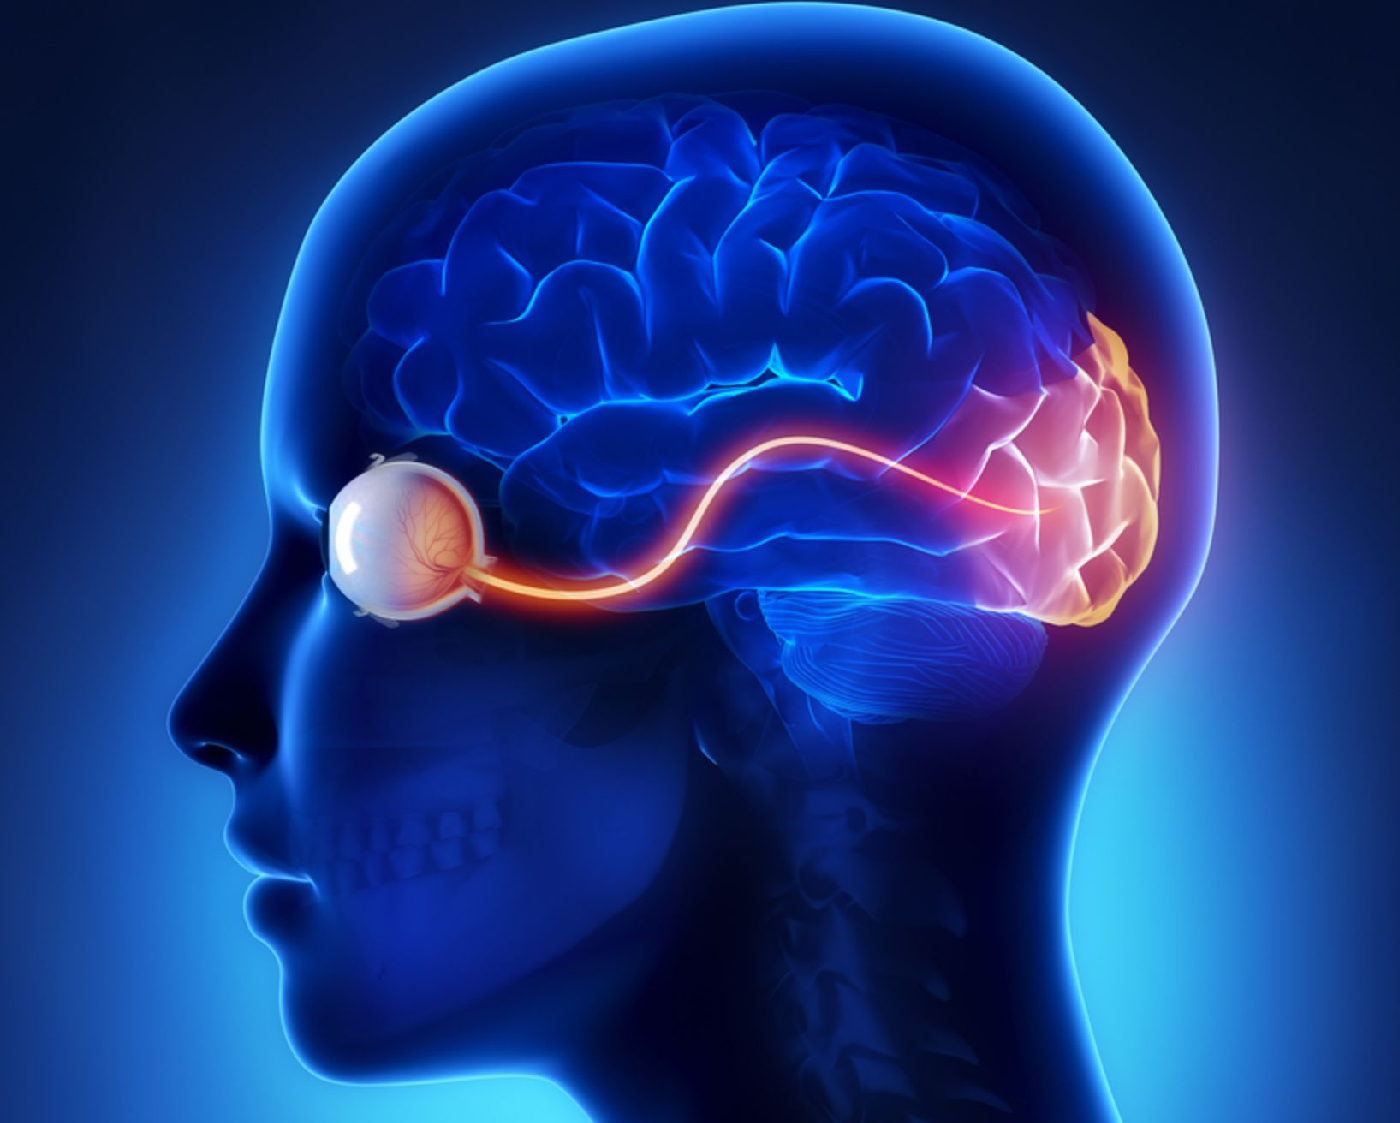
\includegraphics[width=\paperwidth]{images/eye-nerve-brain.pdf}
            };
        \end{tikzpicture}
     \end{frame}
}

%------------------------------------------------

\begin{frame}
\frametitle{Vision}

\Large Vision, of our all senses, is the most powerful and efficient 
{\hilit channel for receiving information} from the physical world.

\end{frame}

%------------------------------------------------

\begin{frame}
\begin{center}
\Huge{\hilit{Why do we create visualizations?}}
\end{center}
\end{frame}

%------------------------------------------------

\begin{frame}
\frametitle{Why do we create visualizations?}

\bi
  \item Map
  \item Record
  \item Abstract
  \item Discover
  \item Clarify
  \item Interact
  \item Communicate
  \item Entertain
\ei

\end{frame}

%------------------------------------------------

\begin{frame}
\frametitle{Maps}
\begin{center}
\ig[width=9cm]{images/konya-map.pdf}

\small{ \lolit{Konya town map, Turkey (c. 6200 BC)}}
\end{center}
\end{frame}

%------------------------------------------------

\begin{frame}
\frametitle{Maps}
\begin{center}
\ig[width=6cm]{images/anaximander-map.pdf}

\small{ \lolit{Anaximander of Miletus (c. 550 BC)}}
\end{center}
\end{frame}

%------------------------------------------------

\begin{frame}
\frametitle{Maps}
\begin{center}
\ig[width=10cm]{images/planetary-movements.pdf}

\small{ \lolit{Planetary Movements (source: wikimedia)}}
\end{center}
\end{frame}

%------------------------------------------------

\begin{frame}
\frametitle{Record}

\begin{columns}[t]
\begin{column}{0.4\textwidth}
\begin{center}
\ig[height=6cm]{images/davinci-drawing1.pdf}

\scriptsize{ {\lolit Leonardo Da Vinci (ca. 1500)}}
\end{center}
\end{column}

\begin{column}{0.5\textwidth}
\begin{center}
\ig[height=6cm]{images/davinci-drawing2.pdf}

\scriptsize{ {\lolit Leonardo Da Vinci (ca. 1500)}}
\end{center}
\end{column}
\end{columns}

\end{frame}

%------------------------------------------------

\begin{frame}
\frametitle{Record}
\begin{center}
\ig[height=7cm]{images/curtis-drawing.pdf}

\small{ \lolit{William Curtis (1746-1799)}}
\end{center}
\end{frame}

%------------------------------------------------

\begin{frame}
\frametitle{Clarify: Stingemore's London Underground (1927)}
\begin{center}
\ig[width=9cm]{images/london-subway-map.pdf}
\end{center}
\end{frame}

%------------------------------------------------

\begin{frame}
\frametitle{Clarify: Harry Beck's London Underground (1933)}
\begin{center}
\ig[width=9cm]{images/beck-underground.pdf}
\end{center}
\end{frame}

%------------------------------------------------

\begin{frame}
\frametitle{Communicate: Hans Rosling}
\begin{center}
\ig[width=10cm]{images/hans-rosling.pdf}
\end{center}
\end{frame}

%------------------------------------------------

\begin{frame}
\frametitle{Entertain: Flight Patterns by Aaron Koblin}
\begin{center}
\ig[width=10cm]{images/flight-patterns.pdf}
\end{center}
\end{frame}

%------------------------------------------------

\begin{frame}
\frametitle{Main functions of visualizations}

\bi
  \item \textbf{Record}: store information
  \bi
    \item photographs, blueprints, sketches, diagrams
  \ei
  \item \textbf{Analyze}: support reasoning about information
  \bi
    \item process and calculate
    \item reason about data
    \item feedback and interaction
  \ei
  \item \textbf{Communication}: convery information to others
  \bi
    \item share and persuade
    \item collaborate and revise
    \item emphasize important aspects of data
  \ei
\ei

{\lolit {\scriptsize based on J. Heer}}

\end{frame}

%------------------------------------------------

\begin{frame}
\begin{center}
\Huge{\hilit{Data Visualization}}
\end{center}
\end{frame}

%------------------------------------------------

{ % all template changes are local to this group.
    \begin{frame}[plain]
        \begin{tikzpicture}[remember picture,overlay]
            \node[at=(current page.center)] {
                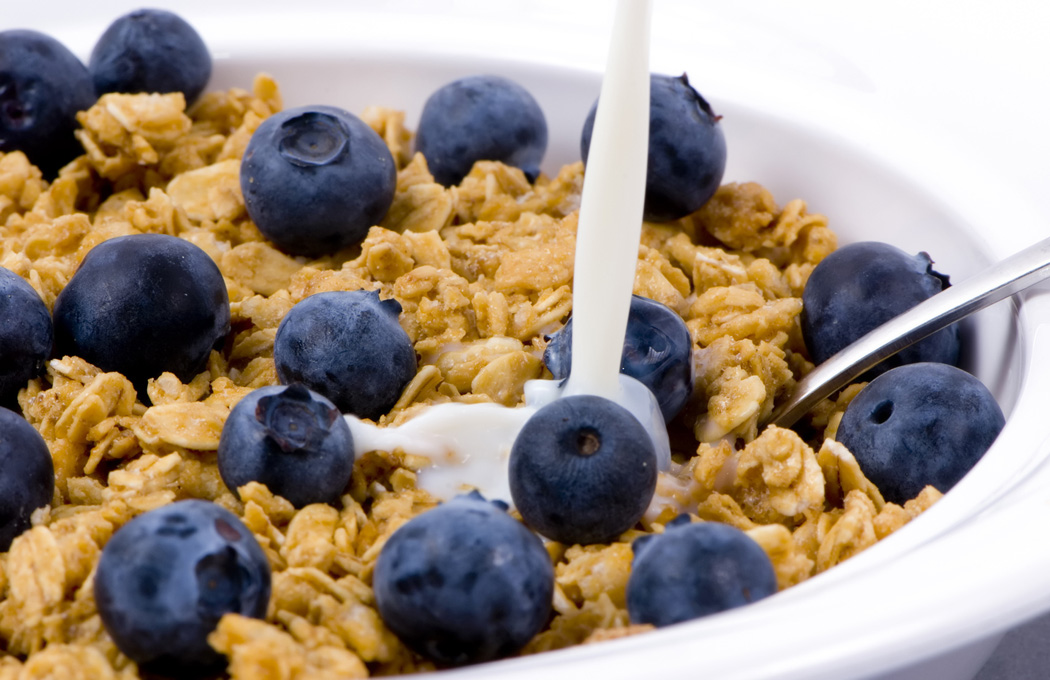
\includegraphics[height=\paperheight]{images/cereals.jpg}
            };
        \end{tikzpicture}
     \end{frame}
}

%------------------------------------------------

\begin{frame}[fragile]
\frametitle{Cereals Data Set}

\begin{columns}[t]
\begin{column}{0.1\textwidth}
%--- empty space ---%
\end{column}
\begin{column}{0.8\textwidth}
\begin{knitrout}\tiny
\definecolor{shadecolor}{rgb}{0.969, 0.969, 0.969}\color{fgcolor}\begin{kframe}
\begin{verbatim}
                 Cups Calories Carbs Fat Fiber Potassium Protein Sodium Sugars
CapnCrunch       0.75      120  12.0   2   0.0        35       1    220     12
CocoaPuffs       1.00      110  12.0   1   0.0        55       1    180     13
Trix             1.00      110  13.0   1   0.0        25       1    140     12
AppleJacks       1.00      110  11.0   0   1.0        30       2    125     14
CornChex         1.00      110  22.0   0   0.0        25       2    280      3
CornFlakes       1.00      100  21.0   0   1.0        35       2    290      2
Nut&Honey        0.67      120  15.0   1   0.0        40       2    190      9
Smacks           0.75      110   9.0   1   1.0        40       2     70     15
MultiGrain       1.00      100  15.0   1   2.0        90       2    220      6
CracklinOat      0.50      110  10.0   3   4.0       160       3    140      7
GrapeNuts        0.25      110  17.0   0   3.0        90       3    179      3
HoneyNutCheerios 0.75      110  11.5   1   1.5        90       3    250     10
NutriGrain       0.67      140  21.0   2   3.0       130       3    220      7
Product19        1.00      100  20.0   0   1.0        45       3    320      3
TotalRaisinBran  1.00      140  15.0   1   4.0       230       3    190     14
WheatChex        0.67      100  17.0   1   3.0       115       3    230      3
Oatmeal          0.50      130  13.5   2   1.5       120       3    170     10
Life             0.67      100  12.0   2   2.0        95       4    150      6
Maypo            1.00      100  16.0   1   0.0        95       4      0      3
QuakerOats       0.50      100  14.0   1   2.0       110       4    135      6
Muesli           1.00      150  16.0   3   3.0       170       4    150     11
Cheerios         1.25      110  17.0   2   2.0       105       6    290      1
SpecialK         1.00      110  16.0   0   1.0        55       6    230      3
\end{verbatim}
\end{kframe}
\end{knitrout}
\end{column}
\begin{column}{0.1\textwidth}
%--- empty space ---%
\end{column}
\end{columns}

\end{frame}

%------------------------------------------------

\begin{frame}
\frametitle{Some questions}

\bbi
  \item Which cereal has the most/lest potassium?
  \item Is there a relationship between potassium and fiber? \\
  If so, are there any outliers?
  \item Which is the ``healthiest'' cereal?
\ei

\end{frame}

%------------------------------------------------

\begin{frame}
\frametitle{Data Visualization}

A key component of computing with data consists of \textbf{Data Visualization}

\end{frame}

%------------------------------------------------

\begin{frame}[fragile]
\begin{center}
\ig[width=10cm]{images/google-datavis.pdf}
\end{center}
\end{frame}

%------------------------------------------------

\begin{frame}
\frametitle{Data Visualization}
\begin{center}
\ig[width=8cm]{images/vis_areas.pdf}
\end{center}
\end{frame}

%------------------------------------------------

\begin{frame}
\frametitle{Data Visualization}

\begin{quotation}
``Data visualization is an umbrella term to cover all types of visual 
representations that support the exploration, examination, and communication
of data.''
\end{quotation}

Stephen Few

\end{frame}

%------------------------------------------------

\begin{frame}
\frametitle{Why data visualizations?}

\bbi
  \item see overall patterns and detailed behavior
  \item reveal patterns
  \item identify trends
  \item identify exceptions and outliers
  \item summarize information
\ei

\end{frame}

%------------------------------------------------

\begin{frame}
\frametitle{Data Visualization}

Data Visualization
\bi
  \item Statistical Graphics?
  \item Computer Graphics?
  \item Computer Vision?
  \item Infographics?
  \item Data Art?
\ei

\end{frame}

%------------------------------------------------

\begin{frame}
\frametitle{Data Visualization}

{\Large We'll focus on concepts and principles to design effective 
statistical graphics and visual displays of data in 
science and technology}

\end{frame}

%------------------------------------------------


\end{document}
